\chapter{ Аналитический раздел}
\label{cha:analysis}

\section{ Цвет}
С физической точки зрения цвет представляет собой свет, который, отражаясь от объекта, попадает в глаз человека. Восприятие цвета человеком может зависить от психологического состояния индивида, от местоположения объекта, от строение глаза человека, от окружаещего света и т.д. То есть восприятяие цвета человеком достаточно субъективно. Свет в свою очередь можно описать как волну, длинна которой возбуждает разные рецепторы человеческого глаза. То есть, индивид будет понимать какого цвета объект перед ним в зависимости от того, в какой диапазон попадет длинна волны света, отраженного от этого объекта.

В какой-то момент необходимо было придумать модель цвета. Описать это явление так, чтобы можно было эффективно и удобно представлять цветовую информацию в цифровом виде. Проблема описания цвета в форме математики была решена еще до появления компьютеров. Одним из первых таких описаний было RGB(Red, green, blue) пространство, идея которого заключалась в представлении всех цветов, различимых человеком, с помощью трех базовых понятий - красного, зеленого и синего. RGB не является одним единственным пространством. Список основных цветовых пространств:
\begin{enumerate}
	\item RGB, sRGB, Adobe RGB
	\item CIEXYZ, CIELAB
	\item CMY(K)
	\item HSL, HSV
\end{enumerate}

$RGB$ -- пространство, строящееся на составление цвета из трех базовых -- красного(Red), синего(Blue) и зеленого(Green). Данную модель часто называют цветовым кубом, потому что каждый базовый параметр цвета, представленного в этой модели, может восприниматься как координата трехмерного пространства.

\begin{figure}[ht!]
	\centering{
		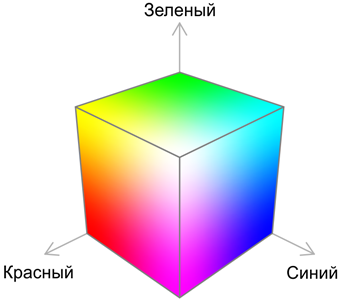
\includegraphics[width=0.4\textwidth]{img/colorCube.png}
		\caption{Представление цветового куба.}}
\end{figure}

Данная модель способна представить 16 777 216(\(2^8 * 2^8 * 2^8\))\\

\textit{CIEXYZ(CIE - International Commission on Illumination)} -- модель, которая является экстраполяцией RGB модели. Данная модель охватывает все цвета, видимые человеком. Когда модель RGB расширили до видимых цветов появились отрицательные числа и чтобы избавиться от них были введены мнимые основные цвета X(мнимый красный), Y(мнимый зеленый), Z(мнимый синий).

\textit{CIELAB(L*a*b*)} -- цветовая модель, которая может отображать цвета за пределами, распознаваемыми человеком. Основывается на трех параметрах: L - яркости(Lightness) и двух цветовых каналов a и b. Проблема данного цветового пространства заключается в том, что расстояние между цветами в этой цветовой модели не соответствует цветовому спектру(Например, расстояние от зеленого к зелено-желтому большое в то время как от красного к синиму достаточно маленькое)

\begin{figure}[ht!]
	\centering{
		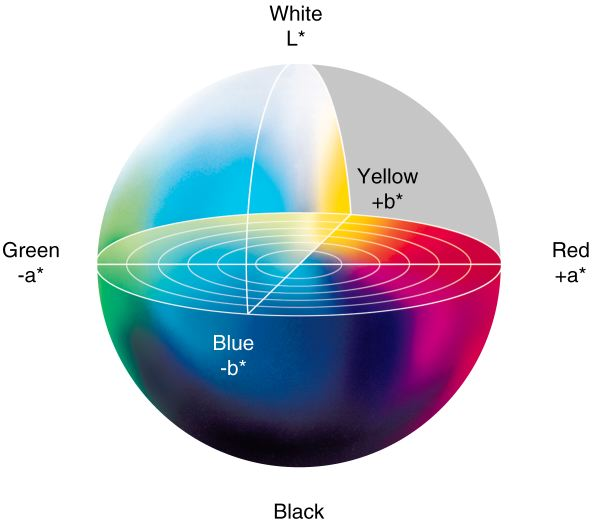
\includegraphics[width=0.4\textwidth]{img/lab.png}
		\caption{Представление цветовой модели CIALAB.}}
\end{figure}

\textit{CMY(K)} -- цветовая модель, аббревиатуру которой можно расшифровать как Cyan(голубой), Magenta(пурпурный), Yellow(желтый), blacK(Key). Данная цветовая модель широко используется в печати документов, изображений. Изначально в данном пространстве исплользовалось только три цвета: cyan, magenta, yellow, с помощью которых можно было получить и черный цвет, смешивая краски. Но это оказалось не эффективно и затратно, поэтому для черного решили ввести отдельный канал, что позволило сэкономить очень много средств.

\begin{figure}[ht!]
	\centering{
		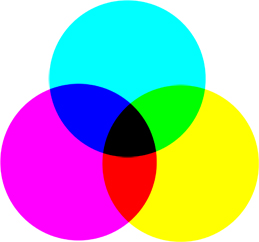
\includegraphics[width=0.4\textwidth]{img/cmyk.png}
		\caption{Представление цветовой модели CIALAB.}}
\end{figure}

\textit{YUV, YIQ} -- цветовые модели, где информация о цвете передавалась в виде яркости(Y) и двху цветоразностных сигналов IQ/UV. Благодаря тому, что в Y изображение хранилось в градациях серого, изображение могло подаваться и на старые бесцветные телевизоры.

\textit{HSL, HSV} -- цветовые пространства, строящиеся на оттенке(Hue), насещенности(Saturation), яркости(Lightness) или значении(Value)

\begin{figure}[ht!]
	\centering{
		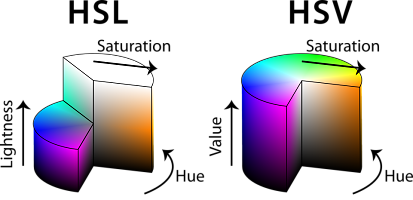
\includegraphics[width=0.4\textwidth]{img/hsl_hsv.png}
		\caption{Представление цветовой модели CIALAB.}}
\end{figure}

\subsection{ Пребладающий цвет}
Стоит выделить понятие преобладающий цвет, которое так часто использовалось выше. Цвет может быть преобладающим чисто математически/физически, а может быть преобладающим с точки зрения человека. Когда мы смотрим на изображение, в котором 70\% черного цвета, а остальные 30\% - яркий выразительный оранжевый оттенок, мы можем выделить как раз таки эти два разных преобладающих цвета. В первом случае мы возьмем преобладающий цвет как нечто физическое и скажем, что в нашем изображении доминирующий цвет - черный, потому что он занимает большую часть картники. А во втором случае рассмотрим преобладающий цвет с точки зрения человека, где скажем, что оранжевый преобладает, потому что наш глаз в первую очередь обратит внимание на более яркую, выразительную точку, чем темную и тусклую.
\subsection{ Квантование цвета}
\subsection{ Цветовые гистограммы}
\subsection{ MPEG-7}
\subsection{ Трехмерное представление цвета}

\section{ Алгоритмы веделения преобладающего цвета}
\subsection{ Histogram algorithms}
\subsection{ GLA(generalized Lloyd Algorithm)}
\subsection{ Clustering algorithms}

\section{ Выбор подходящего алгоритма для решения задачи}
